\section{INVERSE KINEMATICS MODEL AND ANGLE CALCULATION}

\subsection{Manipulator Description}

The arm is a serial RRRR (revolute--revolute--revolute--revolute) manipulator with four actively driven position joints and a gripper. The wrist joint ($\theta_4$) is held fixed throughout the pick-and-place process. Therefore, for the purpose of positioning the gripper tip, the wrist and gripper behave as a single rigid extension of the forearm. The angle $\theta_1$ represents the base rotation angle, $\theta_2$ represents the shoulder movement angle, and $\theta_3$ represents the elbow movement angle.

\begin{table}[htbp]
    \centering
    \caption{Joint configuration of the robotic arm}
    \label{tab:joint_configuration}
    \begin{tabular}{c l l l}
        \toprule
        Joint & Name & Motion Type & Servo \\
        \midrule
        1 & Base & Yaw about vertical axis & DS3218 \\
        2 & Shoulder & Pitch & MG996R \\
        3 & Elbow & Pitch & MG996R \\
        4 & Wrist & Pitch & MG996R \\
        -- & Gripper & Open/close & MG996R \\
        \bottomrule
    \end{tabular}
\end{table}

The main link dimensions used in the kinematic model are given in Table~\ref{tab:link_details}.

\begin{table}[htbp]
    \centering
    \caption{Link dimensions used in the kinematic model}
    \label{tab:link_details}
    \begin{tabular}{c l c}
        \toprule
        Parameter & Description & Value \\
        \midrule
        $H$ & Base to shoulder effective height & 100 mm \\
        $L_1$ & Shoulder to elbow length & 100 mm \\
        $L_2$ & Elbow to gripper tip length & 210 mm \\
        $Z$ & Object height & 40 mm \\
        \bottomrule
    \end{tabular}
\end{table}

\subsubsection{Design Decision: Neutralized Wrist}

Since the prototype has a small pick-and-place workspace and relatively short travel distances, wrist pitching is held at a fixed angle throughout the operation. This fixed angle is represented by $\beta$ for convenience. In the implemented prototype, $\beta=0^\circ$, meaning that the gripper is mounted in line with the forearm.

\begin{figure}[htbp]
    \centering
    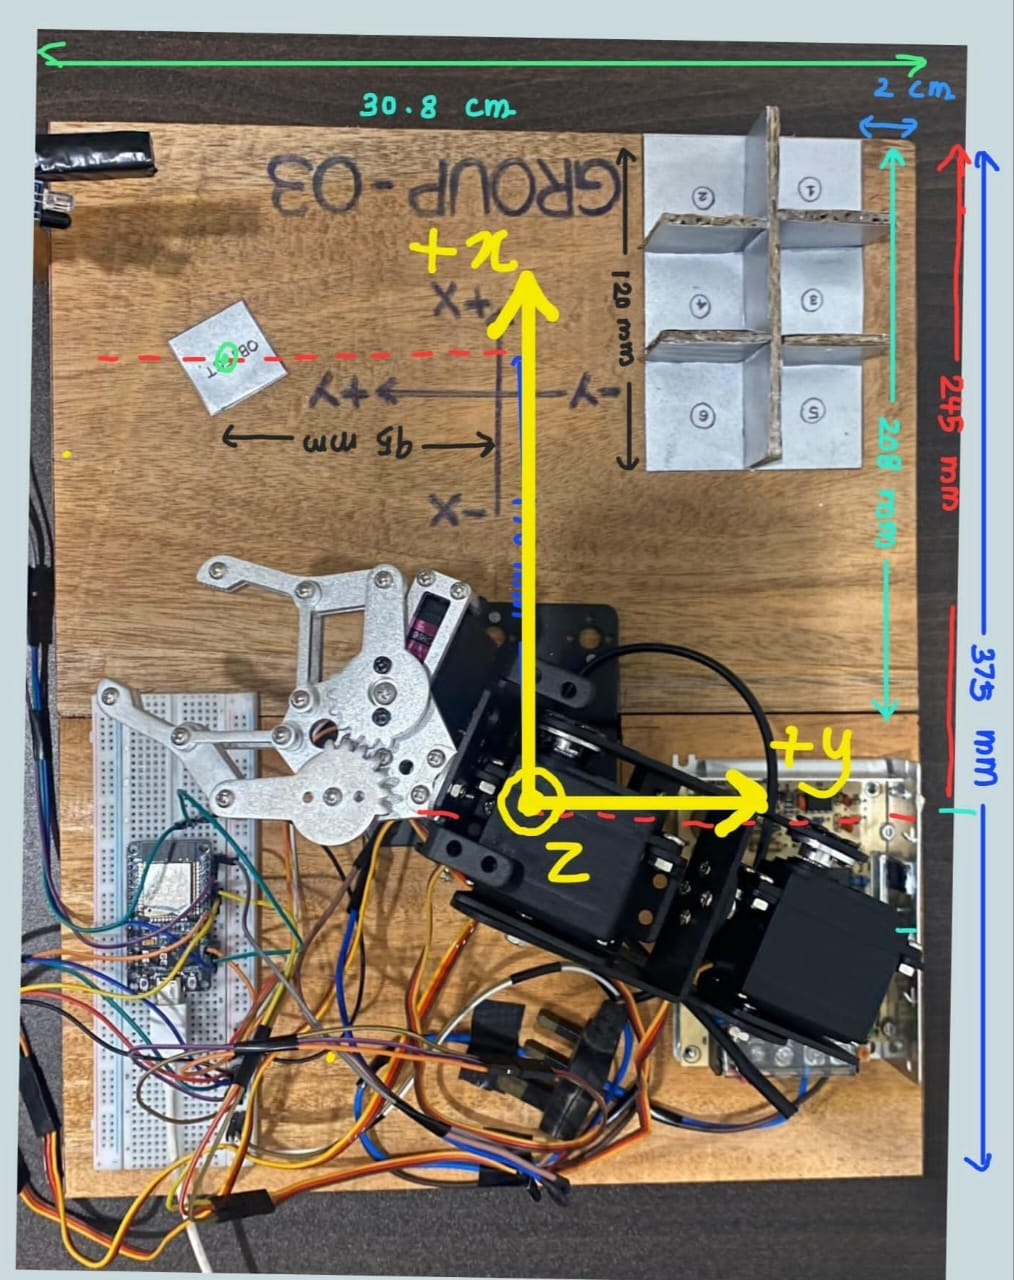
\includegraphics[width=\columnwidth]{figures/Coordinate system.jpeg}
    \caption{Coordinate system and geometric parameters of the robotic arm for inverse kinematics analysis}
    \label{fig:coordinate system}
\end{figure}

\subsubsection{Base Frame Convention}

The base frame convention matches the calibration marks on the physical workspace. The origin is located at the intersection of the base vertical rotation axis and the table surface. The $X$-axis points toward the forward workspace and placement grid, the $Y$-axis represents the lateral direction, and the $Z$-axis is vertical and positive upward.

\subsection{Denavit--Hartenberg Parameters}

The standard Denavit--Hartenberg (DH) convention is used, with the vertical axis of joint 1 and parallel horizontal pitch axes for joints 2--4. The resulting DH parameters are given in Table~\ref{tab:dh_parameters}.

\begin{table}[htbp]
    \centering
    \caption{Denavit--Hartenberg parameters}
    \label{tab:dh_parameters}
    \begin{tabular}{c c c c c}
        \toprule
        $i$ & $a_{i-1}$ & $\alpha_{i-1}$ & $d_i$ & $\theta_i$ \\
        \midrule
        1 & 0 & $0^\circ$ & $H$ & $\theta_1$ \\
        2 & 0 & $90^\circ$ & 0 & $\theta_2$ \\
        3 & $L_1$ & $0^\circ$ & 0 & $\theta_3$ \\
        4 & $L_2$ & $0^\circ$ & 0 & $\theta_4=\beta$ \\
        5 (tool) & $L_g$ & $0^\circ$ & 0 & 0 \\
        \bottomrule
    \end{tabular}
\end{table}

\subsection{Explicit Joint Transformation Matrices}

Using the standard DH convention, the transformation matrix for each joint is expressed as

\begin{equation}
{}^{i-1}A_i =
\begin{bmatrix}
\cos\theta_i &
-\sin\theta_i &
0 &
a_{i-1}
\\
\sin\theta_i\cos\alpha_{i-1} &
\cos\theta_i\cos\alpha_{i-1} &
-\sin\alpha_{i-1} &
-\sin\alpha_{i-1}d_i
\\
\sin\theta_i\sin\alpha_{i-1} &
\cos\theta_i\sin\alpha_{i-1} &
\cos\alpha_{i-1} &
\cos\alpha_{i-1}d_i
\\
0 & 0 & 0 & 1
\end{bmatrix}.
\label{eq:dh_general}
\end{equation}

Substituting the corresponding fixed values of $\alpha_{i-1}$ into the standard DH transformation gives the following explicit transformation matrices.

\subsubsection{Joint 1 -- Base Yaw}

For $\alpha_0=0^\circ$ and $d_1=H$,

\begin{equation}
{}^0A_1 =
\begin{bmatrix}
\cos\theta_1 & -\sin\theta_1 & 0 & 0\\
\sin\theta_1 & \cos\theta_1 & 0 & 0\\
0 & 0 & 1 & H\\
0 & 0 & 0 & 1
\end{bmatrix}.
\label{eq:a1}
\end{equation}

\subsubsection{Joint 2 -- Shoulder Pitch}

For $\alpha_1=90^\circ$ and $a_1=0$,

\begin{equation}
{}^1A_2 =
\begin{bmatrix}
\cos\theta_2 & 0 & \sin\theta_2 & 0\\
\sin\theta_2 & 0 & -\cos\theta_2 & 0\\
0 & 1 & 0 & 0\\
0 & 0 & 0 & 1
\end{bmatrix}.
\label{eq:a2}
\end{equation}

\subsubsection{Joint 3 -- Elbow Pitch}

For $\alpha_2=0^\circ$ and $a_2=L_1$,

\begin{equation}
{}^2A_3 =
\begin{bmatrix}
\cos\theta_3 & -\sin\theta_3 & 0 & L_1\cos\theta_3\\
\sin\theta_3 & \cos\theta_3 & 0 & L_1\sin\theta_3\\
0 & 0 & 1 & 0\\
0 & 0 & 0 & 1
\end{bmatrix}.
\label{eq:a3}
\end{equation}

\subsubsection{Joint 4 -- Wrist Pitch}

The wrist joint is fixed at $\theta_4=\beta$. Therefore, for $\alpha_3=0^\circ$ and $a_3=L_2$,

\begin{equation}
{}^3A_4 =
\begin{bmatrix}
\cos\beta & -\sin\beta & 0 & L_2\cos\beta\\
\sin\beta & \cos\beta & 0 & L_2\sin\beta\\
0 & 0 & 1 & 0\\
0 & 0 & 0 & 1
\end{bmatrix}.
\label{eq:a4}
\end{equation}

The transformation from the base frame to the wrist frame is therefore

\begin{equation}
{}^0A_4 =
{}^0A_1
{}^1A_2
{}^2A_3
{}^3A_4.
\label{eq:a04}
\end{equation}

Since $\theta_4$ is fixed at the constant value $\beta$, the transformation contains only three unknown joint variables, namely $\theta_1$, $\theta_2$, and $\theta_3$. These variables can be determined from the desired gripper-tip position $(X,Y,Z)$ without performing a separate wrist-orientation decoupling step.

\subsection{Forward Kinematics}

Multiplying the transformation chain, the gripper-tip position in the base frame can be expressed using the cumulative pitch angle

\begin{equation}
\phi = \theta_2+\theta_3+\theta_4.
\label{eq:phi}
\end{equation}

The radial distance from the base axis is

\begin{equation}
r =
L_1\cos(\theta_2)
+
L_2\cos(\theta_2+\theta_3)
+
L_g\cos(\phi).
\label{eq:radial}
\end{equation}

The relative vertical displacement from the shoulder axis is

\begin{equation}
z_{\mathrm{rel}} =
L_1\sin(\theta_2)
+
L_2\sin(\theta_2+\theta_3)
+
L_g\sin(\phi).
\label{eq:zrel}
\end{equation}

Therefore, the Cartesian coordinates of the gripper tip are

\begin{align}
X &= r\cos(\theta_1), \label{eq:x_position}\\
Y &= r\sin(\theta_1), \label{eq:y_position}\\
Z &= H+z_{\mathrm{rel}}. \label{eq:z_position}
\end{align}

\subsection{Reduction Under the Neutral Wrist Assumption}

Since $\theta_4$ is held at the fixed constant $\beta$, the effective forearm length used throughout the inverse kinematics derivation is

\begin{equation}
L_2 = 10+11 = 21~\mathrm{cm},
\qquad \beta=0^\circ.
\label{eq:effective_l2}
\end{equation}

With $\beta=0^\circ$, the gripper is collinear with the forearm, allowing the wrist and gripper extension to be treated as a rigid link for position calculation.

\subsection{Inverse Kinematics (Closed Form, Elbow-Up)}

Given a target gripper-tip position $(X,Y,Z)$ in the base frame, the horizontal radial distance is calculated as

\begin{equation}
r = \sqrt{X^2+Y^2}.
\label{eq:ik_r}
\end{equation}

The base rotation angle is obtained using the two-argument arctangent function:

\begin{equation}
\theta_1 = \operatorname{atan2}(X,Y).
\label{eq:ik_theta1}
\end{equation}

The relative vertical position with respect to the shoulder is

\begin{equation}
z_{\mathrm{rel}} = Z-H.
\label{eq:ik_zrel}
\end{equation}

The distance from the shoulder joint to the target position is

\begin{equation}
D = \sqrt{r^2+z_{\mathrm{rel}}^2}.
\label{eq:ik_d}
\end{equation}

The target position is reachable only when

\begin{equation}
|L_1-L_2| \leq D \leq L_1+L_2.
\label{eq:reachability}
\end{equation}

For the dimensions used in this prototype,

\begin{equation}
11~\mathrm{cm} \leq D \leq 31~\mathrm{cm}.
\label{eq:reachability_values}
\end{equation}

Using the law of cosines, the elbow angle is obtained from

\begin{equation}
\cos\theta_3 =
\frac{D^2-L_1^2-L_2^2}
{2L_1L_2}.
\label{eq:cos_theta3}
\end{equation}

For the selected elbow configuration,

\begin{equation}
\theta_3 =
-\cos^{-1}(\cos\theta_3).
\label{eq:theta3}
\end{equation}

The shoulder angle is then calculated as

\begin{equation}
\theta_2 =
\operatorname{atan2}(z_{\mathrm{rel}},r)
-
\operatorname{atan2}
\left(
L_2\sin\theta_3,
L_1+L_2\cos\theta_3
\right).
\label{eq:theta2}
\end{equation}

Finally, the wrist angle remains fixed at

\begin{equation}
\theta_4=\beta.
\label{eq:theta4}
\end{equation}

\subsection{Worked Example -- Picking Position}

The picking position was measured from the base rotation point as

\begin{equation}
X=-9.5~\mathrm{cm},
\qquad
Y=17~\mathrm{cm},
\qquad
Z=4~\mathrm{cm}.
\end{equation}

The radial distance is

\begin{align}
r
&= \sqrt{(-9.5)^2+17^2}\\
&=19.474~\mathrm{cm}.
\end{align}

The base angle is

\begin{align}
\theta_1
&=\operatorname{atan2}(-9.5,17)\\
&=-29.197^\circ.
\end{align}

The negative value indicates that the target is located to the left of the reference direction.

The relative vertical position is

\begin{equation}
z_{\mathrm{rel}}=4-10=-6~\mathrm{cm}.
\end{equation}

Therefore,

\begin{align}
D
&=\sqrt{19.474^2+(-6)^2}\\
&=20.378~\mathrm{cm}.
\end{align}

The elbow angle is calculated using

\begin{align}
\cos\theta_3
&=
\frac{20.378^2-10^2-21^2}
{2(10)(21)}\\
&=-0.2994.
\end{align}

Thus,

\begin{equation}
\theta_3
=
-\cos^{-1}(-0.2994)
=
-107.422^\circ.
\end{equation}

The shoulder angle is obtained from

\begin{equation}
\theta_2 =
\operatorname{atan2}(-6,19.474)
-
\operatorname{atan2}
\left(
21\sin(107.422^\circ),
10+21\cos(107.422^\circ)
\right),
\end{equation}

giving

\begin{equation}
\theta_2=62.379^\circ.
\end{equation}

Therefore, the geometric joint angles at the pick position are approximately

\begin{equation}
\boxed{
\theta_1=-29.2^\circ,\quad
\theta_2=62.4^\circ,\quad
|\theta_3|=107.4^\circ
}
\end{equation}

\subsection{Why Calibrated Servo Angles Were Used Instead of Real-Time IK}

The inverse kinematics calculation described above was performed for all seven target positions, including the picking position and six placing positions. The resulting angles were used as an initial reference for testing the robotic arm. Although the calculated values were close to the required positions, physical calibration was required to obtain accurate servo angles.

A calibration program was therefore used to manually adjust the servo positions for each target location. The final calibrated angles were then hardcoded directly into the firmware. Therefore, both the mathematical inverse kinematics model and the physical calibration process were used to obtain the final joint-angle values.

The use of calibrated angles is suitable for this prototype for the following reasons:

\begin{itemize}
    \item The workspace is relatively small, and the angular variation between one placing slot and another is limited.
    
    \item Since all target positions are fixed, the joint angles do not need to be recalculated during every execution. The calibrated values can instead be stored directly in the firmware, reducing unnecessary ESP32 processing.
    
    \item Using calibrated servo angles reduces the possibility of commanding the robotic arm toward an unreachable position.
    
    \item The servo angles can be manually adjusted according to the actual mechanical configuration of the robotic arm rather than relying only on the ideal mathematical model.
    
    \item Since computer vision is not used for determining the target positions at this stage, repeated real-time inverse kinematics calculations are not required for the fixed target positions.
\end{itemize}

\subsection{Comparison of Calculated Angles with Calibrated Servo Values}

The same inverse kinematics procedure used for the picking position was repeated for each of the six storage slots using their measured $(X,Y)$ coordinates and the same vertical displacement. The calibrated picking position was used as the reference point.

The fixed offsets obtained during calibration were used to convert the calculated geometric joint angles into corresponding servo values. The offsets were

\begin{align}
K &= 60.803^\circ && \text{(base)},\\
c_1 &= 60.803^\circ && \text{(shoulder)},\\
c_2 &= 60.803^\circ && \text{(elbow)}.
\end{align}

These offset values were kept unchanged for all six storage slots. The calculated joint angles and the corresponding calibrated servo values are summarized in Table~\ref{tab:angle_comparison}.

\begin{table*}[htbp]
    \centering
    \caption{Comparison between calculated joint angles and calibrated servo values}
    \label{tab:angle_comparison}
    \begin{tabular}{c c c c c c c}
        \toprule
        Position &
        $\theta_1$ Calculated &
        $\theta_2$ Calculated &
        $\theta_3$ Calculated &
        Base: Calc./Code &
        Shoulder: Calc./Code &
        Elbow: Calc./Code \\
        \midrule
        Pick  & $-29.2^\circ$ & $62.4^\circ$ & $107.4^\circ$ & $90.0^\circ/90^\circ$ & $45.0^\circ/45^\circ$ & $95.0^\circ/95^\circ$ \\
        Slot 1 & $27.1^\circ$ & $36.7^\circ$ & $71.5^\circ$ & $33.7^\circ/38^\circ$ & $19.3^\circ/30^\circ$ & $59.0^\circ/67^\circ$ \\
        Slot 2 & $18.4^\circ$ & $44.0^\circ$ & $82.1^\circ$ & $42.4^\circ/45^\circ$ & $26.7^\circ/40^\circ$ & $69.7^\circ/80^\circ$ \\
        Slot 3 & $31.9^\circ$ & $52.6^\circ$ & $94.2^\circ$ & $28.9^\circ/30^\circ$ & $35.2^\circ/40^\circ$ & $81.7^\circ/85^\circ$ \\
        Slot 4 & $22.1^\circ$ & $60.3^\circ$ & $104.7^\circ$ & $38.7^\circ/40^\circ$ & $42.9^\circ/50^\circ$ & $92.3^\circ/100^\circ$ \\
        Slot 5 & $38.4^\circ$ & $66.5^\circ$ & $112.8^\circ$ & $22.4^\circ/25^\circ$ & $49.1^\circ/55^\circ$ & $100.3^\circ/105^\circ$ \\
        Slot 6 & $27.3^\circ$ & $76.2^\circ$ & $124.6^\circ$ & $33.5^\circ/35^\circ$ & $58.8^\circ/55^\circ$ & $112.2^\circ/109^\circ$ \\
        \bottomrule
    \end{tabular}
\end{table*}

\subsubsection{Discussion of Results}

The difference between the calculated and calibrated base angles is approximately $1^\circ$--$4^\circ$ for the target positions. The close agreement indicates that the horizontal geometry, link lengths, and base rotation direction used in the model are consistent with the physical configuration. The base angle primarily depends on the horizontal position of the target and is independent of the object height.

The shoulder ($\theta_2$) and elbow ($\theta_3$) angles exhibit larger differences, approximately $3^\circ$--$16^\circ$, for the storage slots. These differences can be attributed mainly to practical mechanical and measurement factors rather than to the inverse kinematics formulation itself. The main contributing factors include:

\begin{itemize}
    \item The slot coordinates were measured manually from the physical workspace, which can introduce small measurement errors.
    
    \item The actual link dimensions can differ slightly from the ideal model because of bracket thickness, servo-horn offsets, and mounting tolerances.
    
    \item The mathematical model assumes that the gripper is exactly aligned with the forearm. In practice, a small wrist or gripper offset may exist and can affect the calculated joint angles.
\end{itemize}

Accordingly, the differences between the calculated geometric angles and the calibrated servo values are mainly associated with real-world mechanical tolerances, measurement uncertainties, and the difference between the idealized kinematic model and the physical robotic arm.
\cite{hayat2015robot}